\chapter{Ramsey Theory}

\section{Ramsey Numbers}

We consider arbitrary (non proper) colorings of the edge set of a graph \(G\).
We say that a subgraph \(H\) of \(G\) is \vocab{monochromatic} if all of its edges have the same color.

\begin{proposition} \label{prop:k6-monochromatic-triangle}
    Given any red-blue coloring of the edges of \(K_6\),
    there exists a monochromatic triangle.
\end{proposition}

\begin{proof}
    Consider a vertex \(v\) of \(K_6\).
    By the Pigeonhole Principle, there are at least three edges incident to \(v\) that have the same color.
    Let these edges be \(va\), \(vb\), and \(vc\) and, without loss of generality, assume that they are red.
    If any of \(ab\), \(bc\), or \(ca\) are red, then we have a red triangle.
    Otherwise, all of \(ab\), \(bc\), and \(ca\) are blue, and we have a blue triangle.
\end{proof}

We remark that there exists a red-blue coloring of the edges of \(K_5\) with no monochromatic triangle,
given by the coloring in Figure~\ref{fig:red-blue-coloring-k5}.

\begin{figure}[htbp]
    \centering
    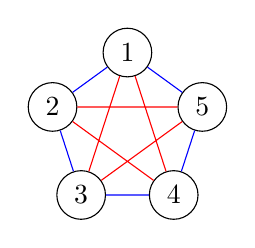
\begin{tikzpicture}
        \foreach \i in {1,...,5} {
            \node[draw, circle] (v\i) at ({72*(\i - 1) + 90}:1) {\(\i\)};
        }
        \draw[blue] (v1) -- (v2) -- (v3) -- (v4) -- (v5) -- (v1);
        \draw[red] (v1) -- (v3) -- (v5) -- (v2) -- (v4) -- (v1);
    \end{tikzpicture}
    \caption{A red-blue coloring of the edges of \(K_5\) with no monochromatic triangle.}
    \label{fig:red-blue-coloring-k5}
\end{figure}

\begin{definition}[Ramsey number]
    Let \(s, t\) be positive integers.
    The \vocab{Ramsey number} \(R(s, t)\) is the smallest integer \(n\) such that any red-blue coloring of the edges of \(K_n\) contains
    a monochromatic red \(K_s\) or a monochromatic blue \(K_t\).
\end{definition}

Note that it is not immediate that \(R(s, t)\) exists for all \(s, t\),
since it is not clear that there is some integer \(n\) with the desired property.
Lemma~\ref{lemma:ramsey-pascal-inequality} shows that \(R(s, t)\) is well-defined.

\begin{example}
    Proposition~\ref{prop:k6-monochromatic-triangle} shows that \(R(3, 3) \leq 6\), and the coloring in Figure~\ref{fig:red-blue-coloring-k5} shows that \(R(3, 3) > 5\),
    so
    \begin{equation}
        R(3, 3) = 6.
    \end{equation}
\end{example}

We remark that 
\begin{equation}
    R(s, t) = R(t, s),
\end{equation}
and
\begin{equation}
    R(s, 2) = s.
\end{equation}

\begin{lemma} \label{lemma:ramsey-pascal-inequality}
    Let \(s, t \geq 3\) be integers.
    Then,
    \begin{equation}
        R(s, t) \leq R(s - 1, t) + R(s, t - 1).
    \end{equation}
\end{lemma}

\begin{proof}
    Let \(n = R(s - 1, t) + R(s, t - 1)\).
    We prove that any red-blue coloring of the edges of \(K_n\) contains a monochromatic red \(K_s\) or a monochromatic blue \(K_t\).
    Consider a red-blue coloring of the edges of \(K_n\).
    Let \(v\) be a vertex of \(K_n\).
    Sicne \(\deg(v) = R(s - 1, t) + R(s, t - 1)\),
    there are at least \(R(s - 1, t)\) edges incident to \(v\) that are red
    or there are at least \(R(s, t - 1)\) edges incident to \(v\) that are blue.

    If there are at least \(R(s - 1, t)\) edges incident to \(v\) that are red,
    then the neighborhood of \(v\) via red edges, \(N_{\textcolor{red}{r}}(v)\),
    induces a subgraph with at least \(R(s - 1, t)\) vertices.
    By the definition of \(R(s - 1, t)\),
    \(N_{\textcolor{red}{r}}(v)\) contains a monochromatic blue \(K_t\),
    or a monochromatic red \(K_{s - 1}\).
    In the former case, we have a monochromatic blue \(K_t\), and hence we are done.
    In the latter case, since all edges between \(v\) and \(N_{\textcolor{red}{r}}(v)\) are red,
    adding \(v\) to the monochromatic red \(K_{s - 1}\) gives a monochromatic red \(K_s\), and hence we are done.

    The case where there are at least \(R(s, t - 1)\) edges incident to \(v\) that are blue is analogous.

    Therefore, any red-blue coloring of the edges of \(K_n\) contains a monochromatic red \(K_s\) or a monochromatic blue \(K_t\), as desired.
\end{proof}

\begin{lemma} \label{lemma:ramsey-binom-inequality}
    Let \(s, t \geq 2\) be integers.
    Then,
    \begin{equation}
        R(s, t) \leq \binom{s + t - 2}{s - 1}.
    \end{equation}
\end{lemma}

\begin{proof}
    The proof is by induction on \(s + t\).
    The base case is when \(s + t = 4\), in which case \(s = t = 2\).
    In this case, \(R(2, 2) = 2 = \binom{2 + 2}{2 - 1}\), so the base case holds.

    Now, suppose that the lemma holds for all pairs of integers \((s', t')\) such that \(s' + t' < s + t\).
    We prove the lemma for the pair \((s, t)\).
    By Lemma~\ref{lemma:ramsey-pascal-inequality}, induction hypothesis, and Pascal's Identity,
    \begin{equation}
        R(s, t) \leq R(s - 1, t) + R(s, t - 1)
        \leq \binom{s + t - 3}{s - 2} + \binom{s + t - 3}{s - 1}
        = \binom{s + t - 2}{s - 1},
    \end{equation}
    as desired.
\end{proof}

The number \(R(s) = R(s, s)\) is called the \vocab{diagonal Ramsey number}.

\begin{corollary}
    For all \(s \geq 2\),
    \begin{equation}
        R(s) \leq \binom{2s - 2}{s - 1} < 2^{2s - 2} = 4^{s - 1}.
    \end{equation}
\end{corollary}

For example, we have that \(R(3) = 6\), \(R(4) = 18\), while \(R(5)\) is only known to be between \(43\) and \(46\).

\textcolor{red}{...}

\begin{definition}
    Let \(G\) and \(H\) be graphs.
    The ramsey number \(r(G, H)\) is the smallest integer \(n\)
    such that any red-blue coloring of the edges of \(K_n\)
    contains a red copy of \(G\) or a blue copy of \(H\).
\end{definition}

\begin{theorem} \label{thm:rGH-lower-bound}
    Let \(G\) and \(H\) be graphs, where \(H\) is connected.
    Then,
    \begin{equation}
        r(G, H) > (\chi(G) - 1)(|V(H)| - 1).
    \end{equation}
\end{theorem}

\begin{proof}
    Let \(m = (\chi(G) - 1)(|V(H)| - 1)\).
    Partition \(V(K_m)\) into parts \(V_1, \dots, V_{\chi(G) - 1}\),
    each of size \(|V(H)| - 1\).

    Color all edges inside each \(V_i\) blue, and all edges between \(V_i\) and \(V_j\) red for \(i \neq j\).
    Then, no blue \(H\) exists because \(H\) is connected and each blue connected component has size at most \(|V(H)| - 1\).

    Suppose that there is a red copy of \(G\).
    Then, the vertex coloring of \(G\) given by assigning each vertex to the index of its part in the partition is a proper coloring of \(G\), with at most \(\chi(G) - 1\) colors, which is a contradiction.

    Therefore, \(r(G, H) > m\), as desired.
\end{proof}

\begin{theorem}[Chvátal] \label{thm:chvatal}
    Let \(n, m\) be positive integers.
    Let \(T_m\) be a tree with \(m\) vertices.
    Then,
    \begin{equation}
        r(T_m, K_n) = (m-1)(n-1) + 1.
    \end{equation}
\end{theorem}

\begin{proof}
    Let \(M = (m-1)(n-1) + 1\).
    By Theorem~\ref{thm:rGH-lower-bound},
    \begin{equation}
        r(T_m, K_n) \geq (\chi(K_n) - 1)(|V(T_m)| - 1) = M.
    \end{equation}

    We show that \(r(T_m, K_n) \leq M\) by induction on \(m + n\).
    If \(m = 2\) or \(n = 2\), the result is straightforward.

    Assume \(n, m \geq 3\),
    and that the result holds
    for all pairs of integers \((n', m')\)
    such that \(n' + m' < n + m\).
    Let \(T_m\) be given.
    Let \(x\) be a leaf of \(T_m\),
    let \(y\) be its unique neighbor,
    and let \(T_{m-1} = T_m - x\).
    Let a red-blue coloring of the edges of \(K_M\) be given.
    Since \(M > (m-2)(n-1) + 1\), by the induction hypothesis,
    there is a red copy of \(T_{m-1}\) or a blue copy of \(K_{n}\).
    If there is a blue copy of \(K_n\), we are done.

    Assume that there is a red copy of \(T_{m-1}\), say \(T^\star \subset K_M\).
    Let \(y^\star\) be the vertex of \(T^\star\) corresponding to \(y\).
    Let \(K = K_M - V(T^\star)\).
    Then,
    \begin{equation}
        |V(K)| = M - (m-1) = (m-1)(n-2) + 1.
    \end{equation}
    Hence, by the induction hypothesis, 
    there is a red copy of \(T_{m}\) or a blue copy of \(K_{n-1}\).
    If there is a red copy of \(T_m\), we are done.
    Assume that there is a blue copy of \(K_{n-1}\), say \(K^\star \subset K_M\).
    If all edges between \(y^\star\) and \(K^\star\) are blue, then adding \(y^\star\) to \(K^\star\) gives a blue copy of \(K_n\), and we are done.
    If there is a red edge between \(y^\star\) and some vertex of \(K^\star\), then adding this edge to \(T^\star\) gives a red copy of \(T_m\), and we are done.
\end{proof}

Recall that the diagonal Ramsey number satisfies the bound
\begin{equation}
    R(s) \geq 2^{\frac{s}{2}},
\end{equation}
although the presented proof is nonconstructive.
It is a major problem to determine constructive bounds for Ramsey numbers.

The bound of \(O(s^2)\) can be obtained constructively,
by considering the graph with \(s-1\) parts of size \(s-1\),
and coloring all edges between different parts red and all edges inside parts blue.
Until 1981, the bet constructive bound was \(O(s^3)\).
We provide a constructive bound of \(O(s^{\log s})\).

\begin{theorem}[Frankl-Wilson] \label{thm:frankl-wilson}
    Let \(n, m, k, s\) be positive integers.
    Let \(p\) be a prime.
    Let \(\mathcal{F}\) be a family of sets of \(k\)-subsets of \([n]\),
    and let \(\mu_0, \mu_1, \dots, \mu_s\) be distinct residues modulo \(p\)
    such that
    \begin{itemize}
        \item \(k \equiv \mu_0 \pmod{p}\),
        \item \(\{\mu_1, \dots, \mu_s\} = \{|B \cap C| \pmod{p} : B, C \in \mathcal{F}\}\),
    \end{itemize}
    Then, \(|\mathcal{F}| \leq \binom{n}{s}\).
\end{theorem}

\begin{proof}
    Clearly, \(s \leq k\). If \(s = k\), then the result is straightforward.
    Assume that \(s < k\).

    Let \(i, j \in [n]\) be numbers such that \(i \leq j\).
    Define the \(\binom{n}{i} \times \binom{n}{j}\) matrix \(N(i, j)\)
    with rows indexed by \(\binom{[n]}{i}\)
    and columns indexed by \(\binom{[n]}{j}\)
    where
    \begin{equation}
        N^{ij}_{AB} =
        \begin{cases}
            1 & \text{if } A \subset B, \\
            0 & \text{otherwise},
        \end{cases}
    \end{equation}
    for all \(A \in \binom{[n]}{i}\) and \(B \in \binom{[n]}{j}\).

    Consider \(N^{sk}\).
    Let \(V\) be the vector space over \(\mathbb{R}\) spanned by the rows of \(N^{sk}\).
    Then, \(V \subset \mathbb{R}^{\binom{n}{k}}\) and \(\dim V \leq \binom{n}{s}\).

    Let \(i \in [n]\) such that \(i \leq s\).
    Consider \( N^{is} N^{sk} \).
    Given \(A \in \binom{[n]}{i}\) and \(C \in \binom{[n]}{k}\),
    \begin{equation}
        (N^{is} N^{sk})_{AC} =
        \#
        \left(
            \text{\(s\)-subsets } B : A \subset B \subset C
        \right)
        =
        \begin{cases}
            \binom{n-i}{s-i} & \text{if } A \subset C, \\
            0 & \text{otherwise}.
        \end{cases}
    \end{equation}
    Therefore,
    \begin{equation}
        N^{is} N^{sk} = \binom{n-i}{s-i} N^{ik}.
    \end{equation}
    Then, each row of \(N^{ik}\) is in \(R^{\binom{n}{k}}\),
    and is a linear combination of the rows of \(N^{sk}\).
    Therefore, the row space of \(N^{ik}\) is a subspace of \(V\),

    Now, consider \(M^{ik} = {N^{ik}}^T N^{ik}\),
    which is a \(\binom{n}{k} \times \binom{n}{k}\) matrix.
    Given \(B, C \in \binom{[n]}{k}\),
    \begin{equation}
        M^{ik}_{BC} = 
        ({N^{ik}}^T N^{ik})_{BC} =
        \#
        \left(
            \text{\(i\)-subsets } A : A \subset B \text{ and } A \subset C
        \right)
        =
        \binom{|B \cap C|}{i}.
    \end{equation}
    Moreover, the rows of \(M^{ik}\) are linear combinations of the rows of \(N^{ik}\), and hence are in \(V\).

    Define \(a_0, a_1, \dots, a_s \in \mathbb{R}\) such that
    \begin{equation}
        \prod_{i=1}^{s} (x - \mu_i) = \sum_{i=0}^{s} a_i \binom{x}{i},
    \end{equation}
    as a polynomial equality, which is possible since
    \(
        \left\{\binom{x}{0}, \binom{x}{1}, \dots, \binom{x}{s}\right\}
    \)
    forms a basis for the space of polynomials of degree at most \(s\).

    Let
    \begin{equation}
        M = \sum_{i=0}^{s} a_i M^{i k},
    \end{equation}
    which is a \(\binom{n}{k} \times \binom{n}{k}\) matrix.
    Given \(B, C \in \binom{[n]}{k}\),
    \begin{equation}
        M_{BC} = \sum_{i=0}^{s} a_i \binom{|B \cap C|}{i} = \prod_{i=1}^{s} (|B \cap C| - \mu_i).
    \end{equation}
    Moreover, the rows of \(M\) are linear combinations of the rows of \(M^{ik}\), and hence are in \(V\).

    Consider the minor \(M^{\mathcal{F}}\) of \(M\)
    indexed by the rows and columns corresponding to the sets in \(\mathcal{F}\).
    Since the rank of \(M\) is at most \(\binom{n}{s}\),
    it follows that the rank of \(M^{\mathcal{F}}\) is at most \(\binom{n}{s}\).
    Given \(B, C \in \mathcal{F}\),
    \begin{equation}
        (M^{\mathcal{F}})_{BC} = \prod_{i=1}^{s} (|B \cap C| - \mu_i) \in \mathbb{Z}.
    \end{equation}
    If \(B \neq C\), then \(M^{\mathcal{F}}_{BC} \equiv 0 \pmod{p}\),
    since \(|B \cap C| \equiv \mu_i \pmod{p}\) for some \(i \in [s]\).
    If \(B = C\), then \(M^{\mathcal{F}}_{BB} \not\equiv 0 \pmod{p}\),
    since \(|B \cap B| = k \equiv \mu_0 \not\equiv \mu_i \pmod{p}\) for all \(i \in [s]\).
    Therefore,
    the matrix \(M^{\mathcal{F}} \pmod{p}\) is a diagonal matrix with non-zero diagonal entries, and hence has non-zero determinant modulo \(p\).
    Thus, \(\det M^{\mathcal{F}}\) is an integer not divisible by \(p\).
    In particular, \(\det M^{\mathcal{F}} \neq 0\).

    Therefore, \(M^{\mathcal{F}}\) is a \(|\mathcal{F}| \times |\mathcal{F}|\) matrix with non-zero determinant and rank at most \(\binom{n}{s}\).
    Then, \(|\mathcal{F}| \leq \binom{n}{s}\), as desired.
\end{proof}

\begin{corollary}[Ray-Chaudhuri--Wilson] \label{cor:ray-chaudhuri-wilson}
    Let \(n, k\) be positive integers.
    Let \(\mathcal{F}\) be a family of sets of \(k\)-subsets of \([n]\).
    Let
    \begin{equation}
        s = \left|
            \left\{
                |B \cap C| : B, C \in \mathcal{F}
            \right\}
        \right|.
    \end{equation}
    Then, \(|\mathcal{F}| \leq \frac{n}{s}\).
\end{corollary}

\begin{proof}
    Let \(p\) be a prime larger than \(k\).
    Theorem~\ref{thm:frankl-wilson} gives the desired result.
\end{proof}

\begin{theorem}[Constructive Ramsey bound] \label{thm:constructive-ramsey-bound}
    Let \(n\) be a positive integer
    and let \(p\) be a prime such that \(p^2 < n\).
    Let \(G\) be  graph with \(V = \binom{[n]}{p^2 - 1}\).
    and edge set
    \begin{equation}
        E = \left\{
            AB : |A \cap B| \not \equiv -1 \pmod{p}
        \right\}.
    \end{equation}
    Let \(t > \binom{n}{p-1}\).
    Then,
    \(G\) has no complete subgraph or independent set with \(t\) vertices.
\end{theorem}

\begin{proof}
    Suppose \(\mathcal{F}\) is the vertex set of a complete subgraph in \(G\).
    Therefore,
    \begin{equation}
        |A \cap B| \not \equiv -1 \pmod{p}
    \end{equation}
    for all \(A, B \in \mathcal{F}\).
    Therefore,
    \begin{equation}
        s = \left|
            \left\{
                |A \cap B| \pmod{p} : A, B \in \mathcal{F}
            \right\}
        \right|
        \leq p-1,
    \end{equation}
    and \(p^2 - 1 \equiv -1 \not \equiv |A \cap B| \pmod{p}\) for all \(A, B \in \mathcal{F}\).
    By Theorem~\ref{thm:frankl-wilson},
    \begin{equation}
        |\mathcal{F}| \leq \frac{n}{p-1}.
    \end{equation}

    Now, suppose \(\mathcal{F}\) is the vertex set of an independent set in \(G\).
    Then,
    \begin{equation}
        |A \cap B| \equiv -1 \pmod{p}
    \end{equation}
    for all \(A, B \in \mathcal{F}\).
    Therefore,
    \begin{equation}
        \{ |A \cap B| : A, B \in \mathcal{F} \} 
        \subset
        \{ p-1, 2p-1, \dots, (p-1)p - 1 \},
    \end{equation}
    and hence
    \begin{equation}
        s = \left|
            \left\{
                |A \cap B| \pmod{p} : A, B \in \mathcal{F}
            \right\}
        \right|
        = p-1.
    \end{equation}
    By Corollary~\ref{cor:ray-chaudhuri-wilson},
    \begin{equation}
        |\mathcal{F}| \leq \frac{n}{p-1}.
    \end{equation}

    In either case, any complete subgraph or independent set in \(G\) has at most \(\frac{n}{p-1} < t\) vertices, as desired.
\end{proof}

\begin{corollary}
    Let \(p\) a sufficiently large prime.
    Let \(s = \binom{p^3}{p - 1}\).
    Theorem~\ref{thm:constructive-ramsey-bound}
    gives a construction of a graph \(G\) with
    \begin{equation}
        V(G) \geq s^{\frac{\log s}{5 \log \log s}}
    \end{equation}
    and no complete subgraph or independent set with \(s\) vertices.
\end{corollary}

It suffices to show that
\begin{equation}
    \binom{p^3}{p^2 - 1} \geq s^{\frac{\log s}{5 \log \log s}}.
\end{equation}

\begin{lemma}
    Let \(1 \leq b \leq a\).
    Then,
    \begin{equation}
        \left( \frac{a}{b} \right)^b \leq \binom{a}{b} \leq \left( \frac{ea}{b} \right)^b.
    \end{equation}
\end{lemma}

\section{Forbidden Subgraph Problem}

\begin{definition}
    Let \(F\) be a graph.
    The \vocab{extremal Turán number} \(T(n, F)\) is the maximum number of edges in a graph on \(n\) vertices that does not contain a copy of \(F\) as a subgraph.
\end{definition}

\begin{example}[Mantel's Theorem]
    \(T(n, K_3) = \left\lfloor \frac{n^2}{4} \right\rfloor\).
\end{example}

The \vocab{Turán problem} is to determine \(T(n, K_r)\) for all \(r \geq 2\).

Given \(n, r\),
the \vocab{Turán graph} \(T_{r-1}(n)\) is the complete \(r-1\)-partite graph on \(n\) vertices with parts as equal as possible,
i.e., each part has size \(\left\lceil \frac{n}{r-1} \right\rceil\) or \(\left\lfloor \frac{n}{r-1} \right\rfloor\).
We write
\begin{equation}
    t_{r-1}(n) = |E(T_{r-1}(n))|.
\end{equation}

\begin{lemma}
    The Turán graph \(T_{r-1}(n)\) is a maximal \(K_r\)-free graph on \(n\) vertices, that is,
    \(T_{r-1}(n)\) is \(K_r\)-free and adding any edge to \(T_{r-1}(n)\) creates a copy of \(K_r\).
\end{lemma}

\begin{proof}
    Since \(T_{r-1}(n)\) is a complete \(r-1\)-partite graph,
    it is \(K_r\)-free.
\end{proof}

\begin{theorem}[Turán's Theorem] \label{thm:turan}
    Let \(n, r\) be positive integers.
    Then,
    \begin{equation}
        T(n, K_r) = t_{r-1}(n),
    \end{equation}
    and the unique \(K_r\)-free graph with \(n\) vertices and \(t_{r-1}(n)\) edges is the Turán graph \(T_{r-1}(n)\).
\end{theorem}

Hence, the Turán graph \(T_{r-1}(n)\) is called an \vocab{extremal graph} for the Turán problem.
Often, when such extremal graph is unique,
it is easier to prove an extremal result by using the extremal graph explicitly.

\begin{proof}[Proof of~\ref{thm:turan}]
    The result is immediate for \(r = 2\).
    Assume \(r \geq 3\).

    If \(n < r\), then \(\ex(n, K_r) = \binom{n}{2} = t_{r-1}(n)\),
    and the uniqueness of the extremal graph is immediate.
    If \(n = r\), then \(\ex(n, K_r) = \binom{n}{2} - 1 = t_{r-1}(n)\),
    and the uniqueness of the extremal graph is immediate.

    Assume \(n \geq r+1\).
    Assume, as an induction hypothesis, that, for all \(m < n\),
    \begin{equation}
        \ex(m, K_r) = t_{r-1}(m)
    \end{equation}
    and the unique extremal graph is \(T_{r-1}(m)\).

    Let \(G'\) be an \(K_r\)-free graph on \(n\) vertices with at least \(t_{r-1}(n)\) edges.
    Let \(G\) be a subgraph of \(G'\) with exactly \(t_{r-1}(n)\) edges.

    Note that, among all graphs with \(n\) vertices and \(t_{r-1}(n)\) edges,
    the Turán graph \(T_{r-1}(n)\) has the largest minimum degree,
    since it is as close to being regular as possible.

    Let \(x\) be a vertex of minimum degree in \(G\).
    Then, 
    \begin{equation} \label{eq:turan-min-degree}
        \begin{aligned}
        |E(G - x)| &= t_{r-1}(n) - \delta(G) \\
                   &\geq t_{r-1}(n) - \delta(T_{r-1}(n)) = t_{r-1}(n-1).
        \end{aligned}
    \end{equation}
    By the induction hypothesis,
    since \(G - x\) is a \(K_r\)-free graph on \(n-1\) vertices with at least \(t_{r-1}(n-1)\) edges,
    it follows that \(G - x\) is isomorphic to \(T_{r-1}(n-1)\).
    Let \(V_1, \dots, V_{r-1}\) be the parts of the partition of \(V(G - x)\) in \(T_{r-1}(n-1)\).
    Moreover, equality in Equation~\ref{eq:turan-min-degree} holds, which implies that
    \begin{equation}
        d(x) = \delta(G) = \delta(T_{r-1}(n)) = 
        t_{r-1}(n-1) - \left\lfloor \frac{n-1}{r-1} \right\rfloor.
    \end{equation}

    Since \(G\) does not contain a copy of \(K_r\),
    there exists a part \(V_i\) of the partition of \(V(G - x)\) such that \(x\) is not adjacent to any vertex in \(V_i\).
    If \(|V_i| > \left\lfloor \frac{n-1}{r-1} \right\rfloor\),
    then \(d(x) < t_{r-1}(n-1) - \left\lfloor \frac{n-1}{r-1} \right\rfloor\),
    which is a contradiction.
    Therefore, \(|V_i| = \left\lfloor \frac{n-1}{r-1} \right\rfloor\),
    and hence by the degree of \(x\),
    \(x\) is connected to all vertices in \(V(G - x) - V_i\).
    Therefore, \(G\) is isomorphic to \(T_{r-1}(n)\).
    Hence, \(G'\) is isomorphic to \(T_{r-1}(n)\), as desired.
\end{proof}

Note that, when \(r-1\) divides \(n\),
\begin{equation}
    t_{r-1}(n)
    =
    \binom{r-1}{2} \left( \frac{n}{r-1} \right)^2
    = \frac{n^2}{2} \frac{r-2}{r+1}.
\end{equation}

In general,
\begin{equation}
    t_{r-1}(n)
    =
    \left( \frac{r-2}{r+1} + o(1) \right)
    \binom{n}{2}.
\end{equation}

\begin{theorem}[Erd\H{o}s-Stone Theorem] \label{thm:erdos-stone}
    Let \(H\) be a graph.
    Then,
    \begin{equation}
        \ex(n, H)
        =
        \left( \frac{\chi(H)-2}{\chi(H)+1} + o(1) \right)
        \binom{n}{2}
    \end{equation}
\end{theorem}

Note that,
for all \(\chi(H) \geq 3\), 
\nameref{thm:erdos-stone} provides the correct order of magnitude for \(\ex(n, H)\), namely, quadratic in \(n\).
For \(\chi(H) = 2\), \nameref{thm:erdos-stone} only provides that \(\ex(n, H)\) is subquadratic in \(n\).
It is an open problem to determine the correct order of magnitude for \(\ex(n, H)\) when \(\chi(H) = 2\), and few graphs \(H\) have the correct order of magnitude known.

For a family \(\mathcal{F}\) of graphs,
the \vocab{extremal number} \(\ex(n, \mathcal{F})\) is the maximum number of edges in a graph on \(n\) vertices that does not contain a copy of any graph in \(\mathcal{F}\) as a subgraph.

\begin{theorem}[Erd\H{o}s-Gallai Theorem] \label{thm:erdos-gallai}
    Let \(\ell \geq 3\).
    Let \(G\) be a graph with \(n\) vertices
    with at least
    \begin{equation}
        \frac{(\ell - 1)(n-1)}{2} + 1
    \end{equation}
    edges.
    Then, \(G\) contains a cycle of length at least \(\ell\).
\end{theorem}

Note that \nameref{thm:erdos-gallai} is equivalent of stating that
\begin{equation}
    \ex(n, \{C_{\ell}, C_{\ell+1}, \dots\}) = \frac{(\ell - 1)(n-1)}{2}.
\end{equation}

\begin{proof}
    We use induction on \(n\).
    When \(n \leq \ell - 1\),
    the result is vacously true.
    Assume \(n \geq \ell\).
    Assume, as an induction hypothesis, that the result holds for all smaller values of \(n\).

    Let \(G\) be a graph with \(n\) vertices and at least \(\frac{(\ell - 1)(n-1)}{2} + 1\) edges.
    If there exists \(x \in V(G)\) such that \(d(x) \leq \frac{\ell - 1}{2}\),
    then
    \begin{equation}
        |E(G - x)| \geq \frac{(\ell - 1)(n-2)}{2} + 1,
    \end{equation}
    and hence by the induction hypothesis,
    \(G - x\) contains a cycle of length at least \(\ell\),
    as desired.

    Therefore, we assume that \(\delta(G) \geq \frac{\ell}{2}\).
    Let \( P = x_1x_2 \ldots x_p \) be a longest path in \( G \) chosen such that its initial vertex has the highest degree among all initial vertices of longest paths in \( G \).
    All neighbors of \( x_1 \) are in \( P \), since otherwise we could extend \( P \).
    If \(x_1x_i \in E(G)\) for some \(i \geq \ell\), then \(x_1x_2 \ldots x_ix_1\) is a cycle of length at least \(\ell\), and we are done.
    Therefore, the neighborhood of \(x_1\) is contained in 
    \begin{equation}
        \{x_2, x_3, \dots, x_{\ell-1}\}.
    \end{equation}
    Let
    \begin{equation}
        W = \{x_i : x_1x_{i+1} \in E(G)\} \subset \{x_1, x_2, \dots, x_{\ell-2}\}.
    \end{equation}

    For each \(x_i \in W\),
    \(x_i\) is the endpoint of a longest path in \(G\),
    with vertex set \(V(P)\),
    namely \(x_ix_{i-1} \ldots x_1x_{i+1} \ldots x_p\).
    Hence, all neighbors of \(x_i\) are in \(P\).
    Again, if \(x_ix_j \in E(G)\) for some \(j \geq \ell\),
    then \(x_ix_{i-1} \ldots x_1x_{i+1} \ldots x_jx_i\) is a cycle of length at least \(\ell\), and we are done.
    Therefore, for all \(x_i \in W\),
    the neighborhood of \(x_i\) is contained in
    \begin{equation}
        \{x_1, x_2, \dots, x_{\ell-1}\}.
    \end{equation}
    Moreover, for all \(x_i \in W\), \(d(x_i) \leq d(x_1)\).

    Let \(k = \min\{\ell - 1, p\}\).
    and let \(Z = \{x_1, x_2, \dots, x_k\}\).
    So, \(\mathcal{N}(W) \subset Z\).
    Then, the number \(e(W)\) of edges of \(G\) incident to \(W\)
    satisfies 
    \begin{equation}
        e(W) = e(W, Z \setminus W) + |E(G[W])|.
    \end{equation}
    Also, by double counting,
    \begin{equation}
        e(W, Z \setminus W) + 2|E(G[W])| = \sum_{w \in W} d(w).
    \end{equation}
    So,
    \begin{align}
        e(w) &= \frac{e(W, Z \setminus W) + \sum_{w \in W} d(w)}{2} \\
             &\leq \frac{|W| |Z \setminus W|}{2} + \frac{d(x_1)|W|}{2} \\
             = \frac{kd}{2} \leq \frac{\ell-1}{2} d.
    \end{align}

    Hence, \(G - W\) has at least 
    \begin{equation}
        \frac{(\ell - 1)(n-|W|-1)}{2} + 1
    \end{equation}
    edges.
    By the induction hypothesis,
    \(G - W\) contains a cycle of length at least \(\ell\),
    as desired.
\end{proof}

\section{Hamiltonian Cycles}

\begin{theorem}[Dirac--Pósa Theorem]
    Let \(G\) be a graph with \(n\) vertices
    in which
    \begin{equation}
        d(x) + d(y) \geq n
    \end{equation}
    for all nonadjacent vertices \(x\) and \(y\).
    Then \(G\) contains a Hamiltonian cycle.
\end{theorem}

\begin{proof}
    Suppose \(G\) has no Hamiltonian cycle.
    Let \(P = x_1x_2 \ldots x_\ell\) be a longest path in \(G\).
    Note that \(d(x) + d(y) \geq n\) for all nonadjacent vertices \(x\) and \(y\)
    guarantees a path of length at most \(2\) between any two vertices in \(P\).
    Hence, \(x_1x_\ell \not\in E(G)\), since otherwise if \(\ell = n\),
    then we get a Hamiltonian cycle, and if \(\ell < n\), then we can extend \(P\)
    (since \(G\) is connected).

    Since \(P\) is longest, \(N(x_1) \subset V(P)\) and \(N(x_\ell) \subset V(P)\).
    Let 
    \begin{equation}
        W = \{x_i : x_{i+1} \in N(x_1)\} \subset V(P).
    \end{equation}
    Since \(|W| = |N(x_1)| = d(x_1)\), \(|N(x_\ell)| = d(x_\ell)\) and \(d(x_1) + d(x_\ell) \geq n\),
    there exists \(x_j \in W \cap N(x_\ell)\), then \(x_1x_2 \ldots x_j x_\ell x_{\ell-1} \ldots x_{j+1}\) is a cycle,
    and then we would be able to find a longer path if this is not Hamiltonian.
\end{proof}

\begin{theorem}[Thomason] \label{thm:thomason}
    Let \(G\) be a graph in with vertex has odd degree.
    Then, every edge of \(G\) is contained in an even number of Hamiltonian cycles.
\end{theorem}

\begin{proof}
    Define a graph \(L\) with vertex set the set of
    Hamiltonian paths \(P\) in \(G - x\) starting at \(y\),
    The edge set of \(L\) is the set of \(PQ\) where
    \begin{equation}
        P = y v_1 v_2 \ldots v_{w-1} v_w v_{w+1} \ldots v_{z-1} v_z
    \end{equation}
    and 
    \begin{equation}
        Q = y v_1 v_2 \ldots v_{w-1} v_w v_z v_{z-1} \ldots v_{w+2} v_{w+1}.
    \end{equation}

    Note that, for each \(P \in V(L)\),
    \begin{equation}
        d_L(P) =
        \begin{cases}
            d_G(z) - 2 \equiv 1 \pmod{2} & \text{if } xz \in E(G), \\
            d_G(z) - 1 \equiv 0 \pmod{2} & \text{if } xz \not\in E(G).
        \end{cases}
    \end{equation}

    Note that a path \(y v_1 v_2 \ldots v_{w-1} v_w v_{w+1} \ldots v_{z-1} v_z\) 
    has odd degree in \(L\) if and only if \(xz \in E(G)\), that is, \(y v_1 v_2 \ldots v_{w-1} v_w v_{w+1} \ldots v_{z-1} v_z x\) is a Hamiltonian cycle in \(G\).

    By the Handshaking Lemma,
    the number of odd vertices in \(L\) is even,
    and consequently, the number of odd edges in \(L\) is even.
\end{proof}

\begin{conjecture}[Sheehan] \label{conj:sheehan}
    For each \(d \geq 3\), every \(d\)-regular Hamiltonian graph has a second Hamiltonian cycle.
\end{conjecture}

Note that Theorem~\ref{thm:thomason} implies the case of odd \(d\) in Conjecture~\ref{conj:sheehan}.
Moreover, it is known that, if the Conjecture is true for \(d = 4\), then it is true for all \(d \geq 3\).

\section{Forbidden Bipartite Subgraph Problem}

Recall that \nameref{thm:erdos-stone} provides the correct order of magnitude for \(\ex(n, H)\) for all graphs \(H\) with chromatic number at least \(3\).
In this section, we investigate the case when \(H\) is a bipartite graph.

\begin{theorem}[Forbidden \(C_4\), Erd\H{o}s]
    \begin{equation}
        \ex(n, C_4) \leq \frac{n^{3/2}}{2} + \frac{n}{4}.
    \end{equation}
\end{theorem}

\begin{proof}
    Let \(G\) be a graph with \(n\) vertices and no \(C_4\) subgraph
    and \(|E(G)| = \ex(n, C_4)\).
    Let's double count the number of \vocab{cherries} in \(G\),
    that is, the number of pairs \((\{x, y\}, z)\) such that \(xz, yz \in E(G)\).
    On the one hand, for every \(2\)-subset \(\{x, y\}\) of \(V(G)\),
    there is at most one vertex \(z\) such that \(xz, yz \in E(G)\),
    since \(G\) has no \(C_4\) subgraph.
    On the other hand, for every vertex \(z\) of \(G\),
    the number of cherries centered at \(z\) is \(\binom{d(z)}{2}\).
    Therefore, 
    \begin{equation}
        \sum_{z \in V(G)} \binom{d(z)}{2} \leq \binom{n}{2}.
    \end{equation}
    By Jensen's inequality,
    \begin{equation}
        n\binom{\frac{2|E(G)|}{n}}{2} \leq \sum_{z \in V(G)} \binom{d(z)}{2}.
    \end{equation}
    Hence,
    \begin{equation}
        \binom{2|E(G)|/n}{2} \leq \frac{n-1}{2},
    \end{equation}
    and solving this quadratic inequality gives the desired result.
\end{proof}

\subsection{Projective Planes}

\begin{definition}
    Let \(q\) be a positive integer.
    A \vocab{projective plane of order \(q\)} consists of a set \(V\) of \vocab{points}, and a set \(\mathcal{P}\) of \vocab{lines},
    where
    \begin{itemize}
        \item \label{def:projective-plane-1} each line contains \(q+1\) points,
        \item \label{def:projective-plane-2} each point lies on \(q+1\) lines,
        \item \label{def:projective-plane-3} each pair of distinct points lies on a unique line,
        \item \label{def:projective-plane-4} each pair of distinct lines intersect at a unique point.
    \end{itemize}
\end{definition}


\begin{theorem}
    Let \((V, \mathcal{P})\) be a projective plane of order \(q\).
    Then,
    \begin{equation}
        |V| = |\mathcal{P}| = q^2 + q + 1.
    \end{equation}
\end{theorem}

\begin{proof}
    Note that items~\ref{def:projective-plane-1} and~\ref{def:projective-plane-2} imply that \(|V| = |\mathcal{P}|\).

    Since each pair of points lies in exactly one line,
    and each line contains exactly \(\binom{q+1}{2}\) pairs of points,
    \begin{equation}
        \binom{|V|}{2} = |\mathcal{P}| \binom{q+1}{2} = |V| \binom{q+1}{2},
    \end{equation}
    and consequently,
    \begin{equation}
        |V| = q^2 + q + 1.
    \end{equation}
\end{proof}

\begin{example}[The Fano Plane]
    The \vocab{Fano plane} is a projective plane of order \(2\),
    with vertex set \(\{1, 2, 3, 4, 5, 6, 7\}\) and line set
    \begin{equation}
        \Big\{
            \{1, 2, 6\},
            \{1, 4, 7\},
            \{1, 3, 5\},
            \{2, 3, 4\},
            \{2, 5, 7\},
            \{3, 6, 7\},
            \{4, 5, 6\}
        \Big\}.
    \end{equation}
\end{example}

\begin{figure}[ht]
    \centering
    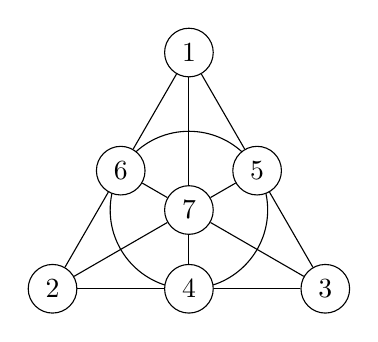
\begin{tikzpicture}[rotate = 90]
        \draw (0, 0) circle (1);
        \node[draw, circle, fill=white] (1) at (0:2) {1};
        \node[draw, circle, fill=white] (2) at (120:2) {2};
        \node[draw, circle, fill=white] (3) at (-120:2) {3};
        \node[draw, circle, fill=white] (4) at (barycentric cs:1=0,2=1,3=1) {4};
        \node[draw, circle, fill=white] (5) at (barycentric cs:1=1,2=0,3=1) {5};
        \node[draw, circle, fill=white] (6) at (barycentric cs:1=1,2=1,3=0) {6};
        \node[draw, circle, fill=white] (7) at (barycentric cs:1=1,2=1,3=1) {7};
        \draw (1) -- (6) -- (2);
        \draw (2) -- (4) -- (3);
        \draw (3) -- (5) -- (1);
        \draw (1) -- (7) -- (4);
        \draw (2) -- (7) -- (5);
        \draw (3) -- (7) -- (6);
    \end{tikzpicture}
    \caption{The Fano Plane}
\end{figure}

The set of \(q\) for which a projective plane of order \(q\) exists is unknown in general.
Proposition~\ref{prop:projective-plane-exists} states that a projective plane of order \(q\) exists for all prime powers \(q\).
Moreover, it is known that there is no projective plane of order \(6\) and \(10\).

\begin{proposition} \label{prop:projective-plane-exists}
    Let \(q\) be a prime power.
    Then, a projective plane of order \(q\) exists.
\end{proposition}

\begin{proof}
    Let \(\mathbb{F}_q\) be the finite field of order \(q\),
    which exists since \(q\) is a prime power.

    Consider the vector space \(\mathbb{F}_q^3\).
    Let \(V\) be the set of \(1\)-dimensional subspaces of \(\mathbb{F}_q^3\).
    Each element of \(V\) has \(q-1\) non-zero vectors, and any two distinct elements of \(V\) have intersection \(\{0\}\).
    Since \(\mathbb{F}_q^3\) has \(q^3 - 1\) non-zero vectors,
    \begin{equation}
        |V| = \frac{q^3 - 1}{q-1} = q^2 + q + 1.
    \end{equation}

    Let \(\mathcal{P}\) be the set of \(2\)-dimensional subspaces of \(\mathbb{F}_q^3\).
    Note that \(\mathcal{P}\) is in bijection with \(V\) by taking the orthogonal complement, hence 
    \begin{equation}
        |\mathcal{P}| = q^2 + q + 1.
    \end{equation}

    As an abuse of notation, we identify a \(2\)-dimensional subspace with the set of \(1\)-dimensional subspaces it contains.
    The number of \(1\)-dimensional subspaces contained in a \(2\)-dimensional subspace is \(\frac{q^2 - 1}{q-1} = q+1\).
    \textcolor{red}{... TBD ...}
\end{proof}

\section{Borsuk's Conjecture}

Let \(S \subset \mathbb{R}^d\).
The \vocab{diameter} of \(S\) is \(\sup_{x, y \in S} \|x - y\|\).
For a set \(S \subset \mathbb{R}^d\),
the \vocab{unit graph} \(U(S)\) of \(S\) is the graph with vertex set \(S\) and edge set \(\{xy : \|x - y\| = 1\}\).

For example, the sphere of radius \(\frac{1}{2}\) has diameter \(1\).
The regular \(n\)-simplex in \(\mathbb{R}^d\), consisting of \(n+1\) vertices such that the distance between any two vertices is \(1\), has diameter \(1\).

\begin{conjecture}[Borsuk's Conjecture (1933)]
    Let \(S \subset \mathbb{R}^n\) of diameter \(1\).
    Then, \(\chi(U(S)) \leq n+1\).
\end{conjecture}

Borsuk's Conjecture is false.

\begin{theorem}[Kahn--Kalai, 1993]
    For all sufficiently large \(n\),
    there exists a set \(S \subset \mathbb{R}^n\) of diameter \(1\) such that \(\chi(U(S)) \geq (1.15)^{\sqrt{n}}\).
\end{theorem}

\begin{proof}
    Let \(p\) be a prime.
    Let \(n = \binom{4p-1}{2}\).
    Let the coordinates of \(\mathbb{R}^n\) be indexed by the edges of the complete graph on \(4p-1\) vertices.
    Let \(\alpha = \left(4p^2 -2p\right)^{-1/2}\).

    For each subset \(X \subset [4p-1]\) of size \(2p\),
    define a vector \(v(X) \in \mathbb{R}^n\) by
    \begin{equation}
        v(X)_e = 
        \begin{cases}
            \alpha & \text{if } e \in E(X, V-X), \\
            0 & \text{otherwise},
        \end{cases}
    \end{equation}
    that is, \(v(X)\) is \(\alpha\) times the indicator vector of the edges between \(X\) and \(V-X\).
    %Write \(\langle X \rangle = E(X, V-X)\).
    LEt
    \begin{equation}
        S = \left\{ v(X) : X \in \binom{[4p-1]}{2p} \right\}.
    \end{equation}

    Let \(X, Y \in \binom{[4p-1]}{2p}\).
    The square of the distance between \(v(X)\) and \(v(Y)\) is
    \begin{align}
        &\mathrel{\phantom{=}} \|v(X) - v(Y)\|^2 \\
        &= \alpha^2 \left| E(X, V-X) \symdiff E(Y, V-Y) \right| \\
        &= \alpha^2 |E(X, V-X)| + |E(Y, V-Y)| - 2|E(X, V-X) \cap E(Y, V-Y)|
    \end{align}
    where \(\symdiff\) denotes the symmetric difference.
    Let \(z = |X \cap Y|\).
    Then, \(2p-z = |X \cap \overline{Y}| = |\overline{X} \cap Y|\),
    and \(z - 1 = |\overline{X} \cap \overline{Y}|\)
    Note that \(E(X, V-X) \cap E(Y, V-Y)\) consists of the edges between \(X \cap Y\) and \(\overline{X} \cap \overline{Y}\), and between \(X \cap \overline{Y}\) and \(\overline{X} \cap Y\).
    Therefore, we compute that 
    \begin{align}
        &\mathrel{\phantom{=}}
        |E(X, V-X)| + |E(Y, V-Y)| - 2|E(X, V-X) \cap E(Y, V-Y)| \\
        &= 2p(2p-1) + 2p(2p-1) - 2\left(z(z-1) + (2p-z)(2p-z-1)\right),
    \end{align}
    which maximizes when \(z = p\), whose value is \(4p^2 - 2p\).
    Therefore, the maximum distance between any two points in \(S\) is \(1\).

    Suppose \(S_0\) is an independent set in \(U(S)\).
    Let \(\mathcal{W} = \{ X \in \binom{[4p-1]}{2p} : v(X) \in S_0 \}\).
    Then, for all distinct \(X, Y \in \mathcal{W}\),
    since \(v(X)\) and \(v(Y)\) are not adjacent in \(U(S)\),
    their distance is smaller than \(1\),
    and consequently, \(|X \cap Y| \neq p\).
    Note that \(|X \cap Y| \neq 0\) and \(|X \cap Y| \neq 2p\).

    Hence, \(\mathcal{W}\) is a set of subsets of \([4p-1]\) such that
    \begin{itemize}
        \item \(|X| = 2p \equiv 0 \pmod{p}\) for all \(X \in \mathcal{W}\),
        \item \(\{ |X \cap Y| \pmod{p} : X, Y \in \mathcal{W} \} \subset \{1, \dots, p-1\}\).
    \end{itemize}
    Therefore, by \nameref{thm:frankl-wilson} Theorem, since \(p - 1 < \frac{4p-1}{2}\),
    we find
    \begin{equation}
        |\mathcal{W}| \leq \binom{4p-1}{p-1}.
    \end{equation}

    Finally,
    \begin{align}
        \chi(U(S)) &\geq \frac{|V(U(S))|}{\binom{4p-1}{p-1}} \\
                   &= \frac{\binom{4p-1}{2p}}{\binom{4p-1}{p-1}} \\
                   &= \frac{(3p)!(p-1)!}{(2p)!(2p-1)!} \\
                   &= \frac{ 3p (3p-1) \cdots (2p)! }{ (2p) (2p-1) \cdots p } > (3/2)^p.
    \end{align}

    But \(n = \binom{4p-1}{2} > \frac{(4p-1)^2}{2}\), which gives \(p > \sqrt{2n}/4\),
    and hence \(\chi(U(S)) > (3/2)^{\sqrt{2n}/4} > (1.154)^{\sqrt{n}}\).

    We have only proved the desired result for \(n\) of the form \(\binom{4p-1}{2}\),
    but for large enough \(n\), we can find the largest prime such that \(n > \binom{4p-1}{2}\) which is not gonna be too far from \(n\) by the Prime Number Theorem.
\end{proof}

\section{The Probabilistic Method}

The typical application of the probabilistic method is to show the existence of an object with certain properties.
The idea is to define a probability space in the set of all objects of interest,
and show that the probability of the object having the desired properties is positive.
All our probability spaces will be finite.

We provide an example of the probabilistic method.
A \vocab{tournament} is an orientation of a complete graph.
Let \(k\) be an integer.
We say a tournament has \vocab{property \(S_k\)} if,
for each \(S \subset V(T)\) with \(|S| = k\), 
there exists \(y \notin S\) such that \(y \to x\) is an arc for all \(x \in S\).

Consider the scenario of organizing a round-robin tournament with \(k\) trophies.
It is undesirable to have a situation where all \(k\) winners have lost to the same participant who did not receive a trophy.
This undesirable property is property \(S_k\).
As an organizer, one aims to avoid tournaments with property \(S_k\), but it is not always possible to do so.

\begin{theorem}
    Let \(k\) and \(n\) be positive integers.
    Assume
    \begin{equation}
        \binom{n}{k} \left( 1 - \frac{1}{2k} \right)^{n-k} < 1.
    \end{equation}
    Then, there exists a tournament on \(n\) vertices with property \(S_k\).
\end{theorem}

Note that \(n > \log 2 k^2 (1 + o(1))\) is a sufficient condition for the assumption to hold.

\begin{proof}
    Define a probability space with \(\Omega\) as the set of tournaments on \([n]\),
    with uniform probability distribution \(\mathbb{P}(T) = 2^{-\binom{n}{2}}\).
    Let \(S \subset [n]\) with \(|S| = k\).
    Define the event \(A_S\) as the event that there is no \(y \notin S\) such that \(y \to x\) for all \(x \in S\).
    Note that the probability that, given \(y \notin S\), \(y \to x\) for all \(x \in S\) is \(\frac{1}{2k}\), and hence
    \begin{equation}
        \mathbb{P}[A_S] = \left( 1 - \frac{1}{2k} \right)^{n-k}.
    \end{equation}

    Therefore, using the Union Bound,
    \begin{equation}
        \mathbb{P}\left[ \bigcup_{|S| = k} A_S \right] \leq \binom{n}{k} \left( 1 - \frac{1}{2k} \right)^{n-k} < 1,
    \end{equation}
    and hence there exists a tournament not in any of the events \(A_S\), that is, a tournament with property \(S_k\).
\end{proof}

\begin{definition}
    A \vocab{real-valued random variable} defined on a probability space \((\Omega, \mathbb{P})\) is a function \(X : \Omega \to \mathbb{R}\).
    The \vocab{expected value of \(X\)} is defined as
    \begin{equation}
        \mathbb{E}[X] = \sum_{\omega \in \Omega} X(\omega) \mathbb{P}(\omega).
    \end{equation}
\end{definition}

Recall that our probability spaces are finite,
and hence the sum is well-defined.
It is sometimes convenient to write the expected value as
\begin{equation}
    \mathbb{E}[X] = \sum_{x \in \mathbb{R}} x \mathbb{P}[X = x].
\end{equation}
Although we are summing over all real numbers,
the sum is finite because \(\mathbb{P}[X = x] = 0\) for all but finitely many \(x \in \mathbb{R}\).

Any operation on \(\mathbb{R}\) is extended to random variables pointwise.
For example, given random variables \(X\) and \(Y\) and real numbers \(a\) and \(b\), the random variable \(aX + bY\) is defined by \((aX + bY)(\omega) = aX(\omega) + bY(\omega)\) for all \(\omega \in \Omega\).

\begin{lemma}[Linearity of Expectation] \label{lem:linearity-of-expectation}
    Let \(X\) and \(Y\) be real-valued random variables defined on a probability space \((\Omega, \mathbb{P})\).
    Then,
    \begin{equation}
        \mathbb{E}[X + Y] = \mathbb{E}[X] + \mathbb{E}[Y].
    \end{equation}
\end{lemma}

\begin{lemma}
    Let \(X\) be a real-valued random variable defined on a probability space \((\Omega, \mathbb{P})\). Then,
    \begin{equation}
        \mathbb{P}[X \geq \mathbb{E}[X]] > 0.
    \end{equation}
\end{lemma}

\begin{proposition}
    Let \(n\) be a positive integer.
    There exists a tournament on \(n\) vertices
    with at least \({n!} 2^{-n+1}\) Hamiltonian paths.
\end{proposition}

\begin{proof}
    Let \(\Omega\) be the set of tournaments on \([n]\),
    with uniform probability distribution, i.e., \(\mathbb{P}(T) = 2^{-\binom{n}{2}}\) for each \(T \in \Omega\).

    For each permutation \(\sigma\) of \([n]\),
    define the random variable \(X_{\sigma}\) by
    \begin{equation}
        X_{\sigma}(T) = 
        \begin{cases}
            1 & \text{if } \sigma(i) \to \sigma(i+1) \text{ is an arc in } T \text{ for all } i \in [n-1], \\
            0 & \text{otherwise}.
        \end{cases}
    \end{equation}
    We compute that
    \begin{equation}
        \mathbb{E}[X_{\sigma}] = 0 \cdot \mathbb{P}[X_{\sigma} = 0] + 1 \cdot \mathbb{P}[X_{\sigma} = 1] = \mathbb{P}[X_{\sigma} = 1] = 
        \frac{2^{\binom{n}{2} - n + 1}}{2^{\binom{n}{2}}} = 2^{-n+1}.
    \end{equation}
    Let \(X = \sum_{\sigma} X_{\sigma}\).
    Then, \(X(T)\) is the number of Hamiltonian paths in \(T\).
    By the Linearity of Expectation (Lemma~\ref{lem:linearity-of-expectation}),
    \begin{equation}
        \mathbb{E}[X] = \sum_{\sigma} \mathbb{E}[X_{\sigma}] = {n!} 2^{-n+1}.
    \end{equation}
    Therefore, there exists a tournament with at least \({n!} 2^{-n+1}\) Hamiltonian paths.
\end{proof}

We say events \(A\) and \(B\) are \vocab{independent} if
\begin{equation}
    \mathbb{P}[A \cap B] = \mathbb{P}[A] \mathbb{P}[B].
\end{equation}
We say that random variables \(X\) and \(Y\) are \vocab{independent} if, for all \(x, y \in \mathbb{R}\), the events \(X = x\) and \(Y = y\) are independent.

\section{Erd\H{o}s--Rényi Model}

Let \(n\) be a positive integer and \(p \in [0, 1]\) be a real number.
The probability space \(\mathfrak{G}(n, p) = (\Omega, \mathbb{P})\) has \(\Omega\) as the set of all graphs on \([n]\),
and \(\mathbb{P}\) defined by
\begin{equation}
    \mathbb{P}[G] = p^{|E(G)|} (1-p)^{\binom{n}{2} - |E(G)|}
\end{equation}
for each \(G \in \Omega\).

Note that
\begin{equation}
    \sum_{G \in \Omega} \mathbb{P}[G]
    = \sum_{\ell=0}^{\binom{n}{2}} \binom{\binom{n}{2}}{\ell} p^{\ell} (1-p)^{\binom{n}{2} - \ell}
    = \left( p + (1-p) \right)^{\binom{n}{2}} = 1,
\end{equation}
and hence \(\mathbb{P}\) is indeed a probability distribution.

Moreover, we can note that, for each edge \(e \in K_{[n]}\), the probability that \(e \in E(\mathfrak{G}(n, p))\) is \(p\), and the probability that \(e \not\in E(\mathfrak{G}(n, p))\) is \(1-p\).
Moreover, all of these events are independent.

For a graph property \(Q\) and a function \(p = p(n)\),
we say that \vocab{almost every \(G \in \mathfrak{G}(n, p)\) has property \(Q\)} if the probability that \(G\) has property \(Q\) tends to \(1\) as \(n \to \infty\).

\begin{lemma}
    Let \(X\) be a non-negative integer-valued random variable on a probability space \((\Omega, \mathbb{P})\).
    Then, \(\mathbb{P}[X = 0] > 1 - \mathbb{E}[X]\).

    In particular,
    if \(X\) is a non-negative integer-valued random variable on \(\mathfrak{G}(n, p)\)
    and \(\mathbb{E}[X] \to 0\) as \(n \to \infty\),
    then \(\mathbb{P}[X = 0] \to 1\) as \(n \to \infty\),
    i.e.,
    almost every \(G \in \mathfrak{G}(n, p)\) has \(X = 0\).
\end{lemma}

\begin{proposition}
    Let \(p = p(n)\) such that \(p(n)n^{2/3} \to 0\) as \(n \to \infty\).
    Then, almost every \(G \in \mathfrak{G}(n, p)\) has no copy of \(K_4\).
\end{proposition}

\begin{proof}
    For each \(S \in \binom{[n]}{4}\), let \(X_S\) be the indicator random variable for the event that \(S\) induces a copy of \(K_4\).
    The expected value of \(X_S\) is
    \begin{equation}
        \mathbb{E}[X_S] = 
        \mathbb{P}[S \text{ induces a copy of } K_4] =
        \prod_{i \neq j \in S} p = p^6.
    \end{equation}
    Let \(X = \sum_{S} X_S\), which is the random variable counting the number of copies of \(K_4\) in \(G\).
    By \nameref{lem:linearity-of-expectation},
    \begin{equation}
        \mathbb{E}[X] = \sum_{S} \mathbb{E}[X_S] = \binom{n}{4} p^6 = o(1) (pn^{2/3})^6 \to 0.
    \end{equation}
    Therefore, almost every \(G \in \mathfrak{G}(n, p)\) has no copy of \(K_4\).
\end{proof}

\section{High Girth and High Chromatic Number}

We proved previously that there are graphs with arbitrarily high chromatic number and no triangles.
Now, we prove that there are graphs with arbitrarily high chromatic number and arbitrarily high girth.

We will determine how small \(p\) must be so that 
\begin{equation}
    \mathbb{P}(\text{\(G\) has at most \(n/2\) cycles of length smaller than \(g\)}) \to 0,
\end{equation}
and how large \(p\) must be so that
\begin{equation}
    \mathbb{P}(\alpha(G) \leq n/2c) \to 0.
\end{equation}
Hopefully, there exists a \(p\) that satisfies both conditions.

\begin{lemma} \label{lem:bounding-short-cycles}
    Let \(g \geq 3\) be fixed.
    Let \(p = p(n) \leq n^{s-1}\), where \(0 < s < 1/(g-1)\).
    Define the random variable \(x\) on \(G \in \mathfrak{G}(n, p)\) as the number of cycles of length smaller than \(g\).
    Then, \(\mathbb{P}[X(G) \geq n/2] \to 0\) as \(n \to \infty\).
\end{lemma}

\begin{proof}
    First, fix \(k\) such that \(3 \leq k \leq g-1\).
    Define \(X_k\) as the random variable counting the number of cycles of length \(k\) in \(G\).
    Then,
    \begin{equation}
        X_k = \sum_{\text{\(k\)-cycle \(C\) in \([n]\)}} X_k^C,
    \end{equation}
    where \(X_k^C\) is the indicator random variable for the event that \(C\) is a cycle in \(G\).
    By \nameref{lem:linearity-of-expectation},
    \begin{equation}
        \mathbb{E}[X_k]
        = \sum_{\text{\(k\)-cycle \(C\) in \([n]\)}} \mathbb{E}[X_k^C] 
        = \frac{n(n-1)\cdots(n-k+1)}{2k} p^k 
        < \frac{n^k}{2k} p^k.
    \end{equation}
    Therefore, since \(X = \sum_{k=3}^{g-1} X_k\), \nameref{lem:linearity-of-expectation} gives
    \begin{align}
        \mathbb{E}[X]
        &< \sum_{k=3}^{g-1} \frac{n^k}{2k} p^k \\
        &\leq \frac{1}{6} n^3p^3 \frac{n^{g-3}p^{g-3} - 1}{np - 1} \\
        &\leq \frac{1}{6} n^3p^3 \frac{n^{g-3}p^{g-3}}{n^{g-3}p^{g-3} - 1} \\
        &\leq n^{g-1}p^{g-1},
    \end{align}
    for all \(n\) sufficiently large.

    Let \(\varepsilon = 1 - s(g-1) > 0\).
    Then, \(\mathbb{E}[X] \leq n^{g-1}p{g-1} = n^{1-\epsilon}\),
    and consequently \(\frac{\mathbb{E}[X]}{n} \to 0\) as \(n \to \infty\).

    Note  that
    \begin{equation}
        \mathbb{E}[X] \geq \frac{n}{2} \mathbb{P}[X \geq n/2],
    \end{equation}
    so
    \begin{equation}
        \mathbb{P}[X \geq n/2] \leq \frac{2\mathbb{E}[X]}{n} \to 0
    \end{equation}
    as \(n \to \infty\).
\end{proof}

\begin{lemma} \label{lem:bounding-independent-number}
    Let \(t\) be an integer such that \(2 \leq t \leq n\).
    Let \(G \sim \mathfrak{G}(n, p)\).
    Then,
    \begin{equation}
        \mathbb{P}[\alpha(G) \geq t]
        \leq \binom{n}{t} (1-p)^{\binom{t}{2}}
        < \left( n e^{-p(t-1)/2} \right)^t.
    \end{equation}
\end{lemma}

\begin{proof}
    Define \(X\) as the random variable counting the number of independent sets of size \(t\) in \(G\).
    Then,
    \begin{equation}
        \mathbb{E}[X] = \binom{n}{t} \left(1-p^{\binom{t}{2}}\right).
    \end{equation}
    Moreover,
    \begin{equation}
        \mathbb{P}[\alpha(G) \geq t]
        = \mathbb{P}[X \geq 1]
        \leq \mathbb{E}[X]
        = \binom{n}{t} \left(1-p^{\binom{t}{2}}\right),
    \end{equation}
    and the result follows using \(\binom{n}{t} < n^t\) and \(1-p \leq e^{-p}\).
\end{proof}

\begin{lemma} \label{lem:bounding-chromatic-number}
    Let \(c\) be a positive integer.
    Let \(p = p(n) \geq 6c \log n / n\).
    Then, 
    \begin{equation}
        \mathbb{P}[\alpha(G) \leq n/2c] \to 0
    \end{equation}
    as \(n \to \infty\).
\end{lemma}

\begin{proof}
    Set \(t = \left\lceil n/2c \right\rceil\) in Lemma~\ref{lem:bounding-independent-number}.
    Then,
    \begin{equation}
        ne^{-p(t-1)/2}
        = ne^{-pt/2} e^{p/2}
        \leq ne^{-3\log n/2} e^{1/2}
        \leq n \cdot n^{-3/2} \to 0,
    \end{equation}
    using that \(pt \geq 3\log n\),
    and the result follows.
\end{proof}

\begin{theorem}[Erd\H{o}s, 1959]
    Let \(c, g\) be positive integers.
    There exists a graph with chromatic number at least \(c\) and girth at least \(g\).
\end{theorem}

\begin{proof}
    Let \(p = p(n)\) such that \(6c \log n / n \leq p \leq n^{s-1}\), where \(0 < s < 1/(g-1)\).
    For concreteness, choose \(p = n^{s-1}\) with \(s = 1/(2g - 2)\).
    By Lemma~\ref{lem:bounding-short-cycles}, almost every \(G \in \mathfrak{G}(n, p)\) has no cycles of length smaller than \(g\).
    By Lemma~\ref{lem:bounding-chromatic-number}, almost every \(G \in \mathfrak{G}(n, p)\) has chromatic number at least \(c\).
    Therefore, almost every \(G \in \mathfrak{G}(n, p)\) has chromatic number at least \(c\) and girth at least \(g\).
    In particular, there exists a graph with chromatic number at least \(c\) and girth at least \(g\).
\end{proof}

\section{The Second Moment Method}

\begin{definition}
    Let \(X\) be a real-valued random variable defined on a probability space \((\Omega, \mathbb{P})\) and mean \(\mu = \mathbb{E}[X]\).
    The \vocab{variance of \(X\)} is defined as
    \begin{equation}
        \operatorname{Var}[X] = \mathbb{E}[(X - \mu)^2].
    \end{equation}
\end{definition}

Note that
\begin{equation}
    \operatorname{Var}[X] = \mathbb{E}[X^2 - 2X\mu + \mu^2] = \mathbb{E}[X^2] - 2\mu^2 + \mu^2 = \mathbb{E}[X^2] - \mu^2.
\end{equation}

The non-negative square root of the variance is called the \vocab{standard deviation} of \(X\).

\begin{lemma}[Chebychev's Inequality]
    Let \(X\) be a real-valued random variable defined on a probability space \((\Omega, \mathbb{P})\) with mean \(\mu = \mathbb{E}[X]\) and standard deviation \(\sigma = \sqrt{\operatorname{Var}[X]}\).
    Then, for all \(t > 0\),
    \begin{equation}
        \mathbb{P}[|X - \mathbb{E}[X]| \geq t\sigma] \leq \frac{1}{t^2}.
    \end{equation}
\end{lemma}

\begin{proof}
    Note that
    \begin{equation}
        \sigma^2
        = \mathbb{E}[(X - \mu)^2]
        = \sum_{r \in \mathbb{R}} r \mathbb{P}[(X - \mu)^2 = r]
        \geq t^2\sigma^2 \mathbb{P}[(X - \mu)^2 \geq t^2\sigma^2],
    \end{equation}
    and the result follows.
\end{proof}

\begin{corollary}
    Let \(X\) be an integer-valued random variable defined on a probability space \((\Omega, \mathbb{P})\) with mean \(\mu = \mathbb{E}[X]\) and standard deviation \(\sigma = \sqrt{\operatorname{Var}[X]}\).
    Then,
    \begin{equation}
        \mathbb{P}[X = 0] \leq \frac{\sigma^2}{\mu^2}.
    \end{equation}
\end{corollary}

\begin{proof}
    Apply Chebychev's Inequality with \(t = \mu/\sigma\)
    to obtain
    \begin{equation}
        \mathbb{P}[X=0] \leq \mathbb{P}[|X - \mu| \geq \mu] \leq \frac{\sigma^2}{\mu^2}.
    \end{equation}
\end{proof}

We showed earlier that if \(pn^{2/3} \to 0\), then almost every \(G \in \mathfrak{G}(n, p)\) has no copy of \(K_4\).
In Proposition~\ref{prop:existence-of-k4}, we will show that if \(pn^{2/3} \to \infty\), then almost every \(G \in \mathfrak{G}(n, p)\) has a copy of \(K_4\).
In other words, if \(p << n^{-2/3}\), then almost every \(G \in \mathfrak{G}(n, p)\) has no copy of \(K_4\), and if \(p >> n^{-2/3}\), then almost every \(G \in \mathfrak{G}(n, p)\) has a copy of \(K_4\).
We call the function \(n^{-2/3}\) the \vocab{threshold function} for the existence of a copy of \(K_4\).

\begin{proposition} \label{prop:existence-of-k4}
    Let \(p = p(n)\) such that \(pn^{2/3} \to \infty\) as \(n \to \infty\).
    Then, almost every \(G \in \mathfrak{G}(n, p)\) has a copy of \(K_4\).
\end{proposition}

\begin{proof}
    Let \(X_S\) be the indicator random variable for the event that \(S\) induces a copy of \(K_4\), where \(S \in \binom{[n]}{4}\).
    Then,
    \begin{equation}
        \mathbb{E}[X_S] = p^{\binom{4}{2}} = p^6.
    \end{equation}
    Let \(X = \sum_{S} X_S\), which is the random variable counting the number of copies of \(K_4\) in \(G\), and consequently
    \begin{equation}
        \mathbb{E}[X] = \binom{n}{4} p^6 > \frac{n^2p^6}{48},
    \end{equation}
    for large enough \(n\).

    We want to estimate \(\sigma^2/\mu^2\), where \(sigma^2 = \mathbb{E}[X^2] - \mu^2\).
    Therefore, we need to estimate \(\mathbb{E}[X^2]\).

    We have
    \begin{equation}
        \mathbb{E}[X^2] = \sum_{S, T \in \binom{[n]}{4}} \mathbb{E}[X_S X_T].
    \end{equation}
    Note that \(X_S X_T = 1\) if and only if \(S\) induces a copy of \(K_4\) and \(T\) induces a copy of \(K_4\).
    However, such value is not constant across all \(S, T \in \binom{[n]}{4}\);
    it depends on the relative positions of the vertices in \(S\) and \(T\).
    We have
    \begin{equation}
        \mathbb{E}[X_S X_T] = p^{12 - \binom{|S \cap T|}{2}}
        = \begin{cases}
            p^{12} & \text{if } |S \cap T| \in \{0, 1\}, \\
            p^{11} & \text{if } |S \cap T| = 2,\\
            p^{9} & \text{if } |S \cap T| = 3,\\
            p^{6} & \text{if } |S \cap T| = 4.
        \end{cases}
    \end{equation}
    Let \(m(j)\) denote the number of pairs \(S, T \in \binom{[n]}{4}\) such that \(|S \cap T| = j\).
    Then,
    \begin{equation}
        m(j) = \binom{n}{4} \binom{4}{j} \binom{n-4}{4-j}.
    \end{equation}

    Using these, we calculate that
    \begin{equation}
        \frac{\sigma^2}{\mu^2} = \frac{\mathbb{E}[X^2] - \mu^2}{\mu^2} \to 0
    \end{equation}
    as \(n \to \infty\).
    Hence, \(\mathbb{P}[X = 0] \to 0\) as \(n \to \infty\), as required.
\end{proof}